\documentclass[conference,compsoc]{IEEEtran}

% *** CITATION PACKAGES ***
%
\ifCLASSOPTIONcompsoc
  \usepackage[nocompress]{cite}
\else
  % normal IEEE
  \usepackage{cite}
\fi

%######### citações modelo abnt 2 ############
\usepackage[num]{abntex2cite}


% *** GRAPHICS RELATED PACKAGES ***
%
\ifCLASSINFOpdf
   \usepackage[pdftex]{graphicx}
  % declare the path(s) where your graphic files are
   \graphicspath{{../pdf/}{../jpeg/}}
  % and their extensions so you won't have to specify these with
  % every instance of \includegraphics
   \DeclareGraphicsExtensions{.pdf,.jpeg,.png}
\else
  % or other class option (dvipsone, dvipdf, if not using dvips). graphicx
  % will default to the driver specified in the system graphics.cfg if no
  % driver is specified.
   \usepackage[dvips]{graphicx}
  % declare the path(s) where your graphic files are
   \graphicspath{{../eps/}}
  % and their extensions so you won't have to specify these with
  % every instance of \includegraphics
   \DeclareGraphicsExtensions{.eps}
\fi

\usepackage{graphics, graphicx}
\usepackage{subfig}
%\usepackage{subfigure}

% correct bad hyphenation here
\hyphenation{op-tical net-works semi-conduc-tor}

% Acentuação Português do Brasil
\usepackage[utf8]{inputenc}

% Permite que o \LaTeX\ fale em português
\usepackage[brazil]{babel}

%hiperlink de Internet
\usepackage[pdftex]{hyperref}


% Conta o número de páginas
\usepackage{lastpage}
\usepackage{setspace}
\pagestyle{plain}

% escrevendo algoritmos
\usepackage[portuguese,ruled,linesnumbered]{algorithm2e}

\begin{document}
%

\title{ANÁLISE DE COMPORTAMENTO DO SISTEMA RODOVIÁRIO NO NORDESTE DO BRASIL PARA PREDIÇÃO DE ROTAS: UMA ABORDAGEM DE MINERAÇÃO DE DADOS}


% author names and affiliations
% use a multiple column layout for up to three different
% affiliations
\author{\IEEEauthorblockN{Othon L. T. Oliveira}
\IEEEauthorblockA{Mestrando em Engenharia de Sistemas\\
Universidade de Pernambuco\\
Email: olto@ecomp.poli.br}
\and
\IEEEauthorblockN{Fernando B. L. Neto}
\IEEEauthorblockA{Universidade de Pernambuco\\PhD - UK\\
Email: fbln@ecomp.poli.br}
}

% conference papers do not typically use \thanks and this command
% is locked out in conference mode. If really needed, such as for
% the acknowledgment of grants, issue a \IEEEoverridecommandlockouts
% after \documentclass


% make the title area
\maketitle

% As a general rule, do not put math, special symbols or citations
% in the abstract
\begin{abstract}
Esse artigo é um recorte de uma dissertação de mestrado, que
teve por objetivo propor e testar conceitos para uma plataforma auto-adaptável que contemple um modelo preditivo de comportamento das
rodovias federais que atravessam o estado de Pernambuco na região Nordeste do Brasil, de modo que seja possível antecipar eventos
que poderão causar constrangimentos, como retenção, redução de fluxo de tráfego. 
Para a proposição desse artigo, foram contempladas informações a partir de 2007 na base de dados da Polícia
Rodoviária Federal de Pernambuco considerando veículos, traçado da via e trechos da rodovia relacionados a acidentes, dentre outros.
Com base nas informações obtidas, foi realizada uma Mineração de Dados utilizando a
metodologia CRISP-DM para encontrar padrões comportamentais nas rodovias e em seu
entorno. Foram empregadas algoritmos de aprendizagem de máquina para classificação e regressão, sendo priorizado, para esse artigo, 
Árvores de Decisão C4.5, implementadas em duas ferramentas: Knime e Weka. Os valores da área sob a curva Roc (AUC) foi 0.7 e da Weca xx.(FALAR SOBRE CONFIABILIDADE)
O modelo de predição
proposto significa um avanço em termos de mobilidade e gestão do
transporte de cargas, uma vez que possibilita antecipar eventos e
comportamentos, favorecendo a escolha de rotas alternativas e
ampliando o espaço temporal de escolha para determinadas rotas.
\end{abstract}

\vspace{0.1cm}

\textbf{Palavras-chave: Modelo de predição, Mineração de dados, Tráfego em rodovias, Árvores de decisão, CRISP-DM.}


\vspace{0.1cm}

\textit{Abstract -- This paper intends to make an explanation ...}

\textit{Keywords: Prediction Model, Data Mining, CRISP-DM, Forecasting the road traffic and Stoppages}




% For peer review papers, you can put extra information on the cover
% page as needed:
% \ifCLASSOPTIONpeerreview
% \begin{center} \bfseries EDICS Category: 3-BBND \end{center}
% \fi
%
% For peerreview papers, this IEEEtran command inserts a page break and
% creates the second title. It will be ignored for other modes.
\IEEEpeerreviewmaketitle



\section{Introdução}

O transporte
de cargas que atravessa as regiões metropolitanas das grandes cidades brasileiras é realizado principalmente pelas rodovias
federais. Essas rodovias frequentemente se encontram congestionadas
em determinados dias e/ou horários. Além do mais, tem sido
contabilizado um aumento expressivo de veículos que por elas
trafegam, a cada ano. No entorno de tais rodovias, particularmente em
perímetros urbanos, comunidades realizam bloqueios para protestar
contra acidentes, atropelamentos ou ainda paralisações de cunho
político, como greves, etc. A proximidade das rodovias de trechos
com morros, florestas, rios, contribuem para que questões ligadas às
intempéries da natureza, como, por exemplo, deslizamentos,
promovam bloqueio das estradas. Essas variáveis impõem constantes
paralisações às rodovias, representando atrasos na entrega, custos
adicionais às empresas e prejuízos de várias ordens.
Tais questões podem ser identificadas em todo o Brasil, no entorno das grandes cidades e rodovias mais utilizadas. 
O estado de Pernambuco, localizado na região Nordeste do Brasil, possuía, em 2015, uma frota de 2.765.521 de veículos, 
sendo que boa parte dessa frota trafega pelas rodovias que cruzam o estado. 
Fora do perímetro urbano as rodovias atravessam outras localidades
com problemáticas diversas, tais como, a precariedade da pavimentação, traçados inapropriados e outras intempéries que
causam, frequentemente, acidentes. A Polícia Rodoviária Federal e
outros órgãos de controle público atendem e registram esses acontecimentos em boletins diários.
A solução para absorver parte dessas informações
requer o estabelecimento de várias etapas, para além da proposição de algumas técnicas de
mineração dos dados. Nesse artigo discutiremos a proposição de uma
solução peculiar, encontrada a partir do estudo original, desenvolvido
no âmbito do Mestrado em Engenharia de Sistemas, para a definição dos dias, horários e rotas, escolhidos por critérios
cientificamente estudados. Isso poderá ser de suma importância para
solucionar a problemática do tráfego em rodovias, particularmente o transporte de carga nas regiões 
do estado de Pernambuco, permitindo fornecer a informação que se faz
necessária para acompanhar veículos, como por exemplo
caminhões, na transposição dos obstáculos que possam surgir ao
transitar pelo estado, conduzindo-os até seu destino de maneira
segura e no menor tempo possível.
O tópico a seguir tratará da discussão das bases teóricas sobre as quais
o estudo se constituiu, sendo, em seguida, apresentada a metodologia
proposta para o seu desenvolvimento e os resultados preliminares
encontrados.



\section{Fundamentação Teórica}

\subsection{Mineração de dados}

No processo de extração do conhecimento (KDD), um dos
importantes passos a ser considerado é a mineração de dados, que se
caracteriza pela aplicação de algoritmos específicos para descoberta de
padrões e/ou comportamentos em grandes bases de dados, também
conhecido como repositórios de dados \cite[Fayyad]{Fayyad}.

A mineração se distingue das técnicas estatísticas pelo fato de que não
trabalha com dados hipotéticos, mas se apoia nos próprios dados para
extrair os padrões (CASTANHEIRA, 2008).
FAYYAD (1996), destaca que é necessário distinguir claramente
KDD e mineração de dados. Enquanto que o primeiro é um processo, a
mineração é um passo no interior desse processo. Todavia, esse passo
é de considerável relevância para que se possa extrair conhecimento
adequadamente. A aplicação “cega” dos métodos de mineração de
dados, ainda segundo Fayyad (1996), pode conduzir à descoberta de
dados sem significado e padrões inválidos.
Existem vários tipos de dados e informações nesses repositórios que
podem ser minerados, contudo esses dados, inicialmente são
selecionados e agrupados, em seguida passam por uma fase de
preprocessamento, que consiste em tratá-los de forma a prepará-los
para a mineração. Essa fase é de fundamental importância na
estruturação dos dados, uma vez que em grandes volumes de dados,
também conhecido “Datawarehouse”, podem existir inconsistências,
faltas (missing data) ou duplicidade e erros de informações.
Nesse sentido, as técnicas de mineração de dados trabalham com
dados estruturados, preenchidos em sua totalidade sem ``missing data'',
para poder extrair informações relevantes. Existem várias maneiras de
 contornar os dados ausentes, como o preenchimento dos dados
através de técnicas de inteligência artificial, da média dos valores,
quando dados numéricos, ou com a moda, quando os dados forem
categóricos. Para cada tipo de dados existem técnicas apropriadas para
serem aplicadas sobre eles, algumas mais sensíveis às problemáticas
elencadas anteriormente e outras mais robustas \cite{DataMining2}, que por sua vez
estão associadas a classes de problemas que a mineração trata.
O processo para extração conhecimento é longo. 
Na figura a seguir temos a ilustração desse caminho:

\begin{figure}[!ht]
\centering
\caption{Fases da mineração de dados até extração do conhecimento}
\flushleft
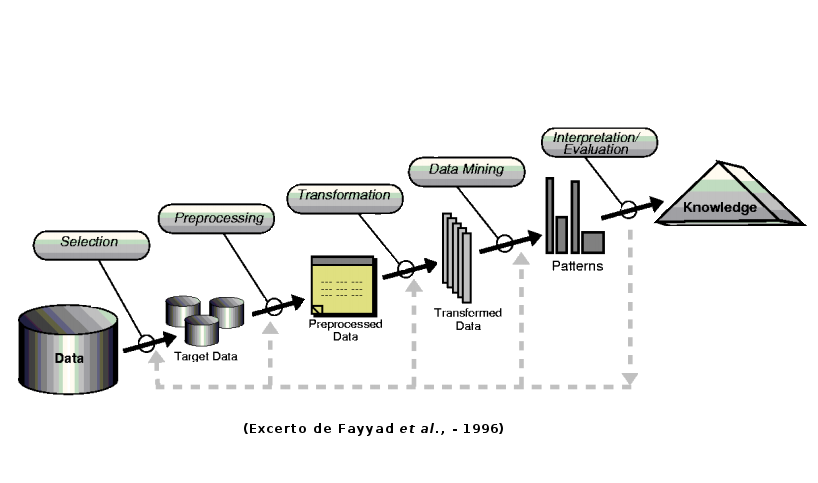
\includegraphics[width=90mm, height=75mm]{Figuras/FayyadSemFundo.png}
\end{figure}


A origem dos dados, os “inputs”, estão representados na figura onde se
lê “Data”, que podem conter ``missing data'' e/ou dados não estruturados. O balão onde se lê
“Selection” representa a coleta das informações ou a seleção dos
dados. Em nossa pesquisa esses dados são provenientes
das mais diversas fontes, tais como, base de informações de acidentes e interdição da Polícia Rodoviária Federal (PRF). 
Dados relevantes podem ser armazenados em “Target Data” com tecnologia
apropriada, utilizando-se técnicas para ler os fluxos de
dados (stream data).
No balão ``Preprocessing'' os dados não-estruturados são tratados, por
exemplo, retirando os missing data. Para estruturar as informações é
preciso utilizar técnicas linguísticas (10). Esses dados normalmente são coletados por técnicas de
Mineração: técnicas de IA como ``Machine Learning'' têm sido comumente
utilizadas. A ``Transformation'' é caracterizada pela estruturação dos dados, que 
podem ser armazenados em Bancos de Dados, conhecidos como ``Datawarehouse''.
O processo de Mineração dos dados começa no balão “Data Mining”,
onde são aplicadas as técnicas de IA conhecidas como classificadores,
para extração de padrões, tais como: ``Decision Tree'' (Árvore de
decisão), ``Artificial Neural Network'' (Redes neurais artificiais),
``Logistic Regression'' (Regressão Logística) e ``Deep Learning'' entre outras.
Algumas técnicas de mineração de dados são fortemente
influenciadas pelas informações na entrada (inputs), como as Árvores
de decisão (11). As Redes Neurais, dependendo da quantidade de
variáveis de entrada, poderão ter milhares de neurônios na camada
intermediária, o que inviabilizaria essa meta-heurística.
Todas as etapas descritas na figura são recorrentes, como indicam
as setas pontilhadas que retornam aos passos anteriores. Utilizar
técnicas de mineração de dados, além de extrair dados, extrai
conhecimento e, com isso, predizer resultados futuros na
saída do modelo, em decorrência dos dados na entrada (12).
Essa técnica de extração de conhecimento chama-se ``Knowledge
Discovery Databases'' (KDD).


\subsection{O CRISP-DM}

O “CRoss Industry Standard Process for Data Mining” – CRISP-DM
é um processo de mineração de dados que descreve como especialistas
nesse campo aplicam as técnicas de mineração para obter os melhores
resultados (1). O CRISP-DM é um processo recursivo, em que cada
etapa deve ser revista até quando o modelo apresentar os resultados
satisfatórios, preliminarmente definidos. O Analista de Dados ou o
Cientista de Dados é o profissional que acompanha e executa o
processo.
O contexto da aplicação do CRISP-DM \cite{Crisp2000} é guiado desde o nível 
mais genérico até o nível mais especializado, sendo normalmente
explicado em quatro dimensões:

\begin{itemize}
 \item O domínio da aplicação -- a área específica que o projeto de mineração de dados acontece;
 \item O tipo de problema -- descreve as classes específicas do objetivo do projeto de mineração de dados;
 \item Os aspectos técnicos -- cobrem as questões específicas como os desafios usualmente encontrados durante o processo de mineração de dados; 
 \item As ferramentas e técnicas -- dimensão específica que cada ferramenta/técnica de mineração de dados é aplicada durante o projeto.
\end{itemize}

A tabela a seguir resume e exemplifica essas dimensões no contexto de aplicação do CRISP-DM.

\begin{table}[!ht]

\caption{Mineração de dados -- contexto de aplicação \cite{Chapman2000}}
\vspace{1mm}
\centering
\begin{tabular}{c|c|c|c}
\textbf{Dimensão} & \textbf{Domínio da} & \textbf{Tipo de } & \textbf{Ferramentas } \\
		  & \textbf{aplicação}  & \textbf{Problema} & \textbf{e Técnicas}   \\ \hline
\textbf{Exemplo}  & Modelo de           & Descrição e       & Clementine  \\
                  & resposta            & sumarização       &             \\ \hline
      --- 	  & Predição            & Segmentação       & MineSet     \\
         	  & agitada             &                   &             \\ \hline
      ---         & ---                 & Descrição do      & Árvore de   \\
                  &                     & conceito          & decisão     \\ \hline
      ---         & ---                 & Classificação     & ---         \\ \hline
      ---         & ---                 & Predição          & ---         \\ \hline
      ---         & ---                 & Análise de        & ---         \\
                  &                     & dependências      & \\            
\\
\end{tabular}
\tiny Fonte: CRISP-DM -- 1.0
\end{table}

A aplicação das técnicas de mineração de dados identifica padrões
ocultos nos dados, inacessíveis pelas técnicas tradicionais, como por
exemplo, consultas em banco de dados, técnicas estatísticas, dentre
outras. Além disso, possibilita analisar um grande número de variáveis
simultaneamente, o que não acontece com o cérebro humano (7), bem
como, com outras técnicas.
Fayyad (8) destaca a natureza interdisciplinar do
KDD que contempla a intersecção de campos de pesquisa tais como
Aprendizagem de Máquina (Machine Learning), Reconhecimento de
Padrões, I.A., estatística, computação de alto desempenho e outros.
Propõe, ainda, que o objetivo principal é extrair um conhecimento de alto
nível a partir de dados de baixo nível, num contexto de grandes bases
de dados. O CRISP-DM, por sua vez, engloba todos esses elementos, como pode ser visto na figura a seguir:

\begin{figure}[!ht]
\centering
\caption{Domínio das técnicas aplicadas a mineração de dados}
\vspace{1mm}
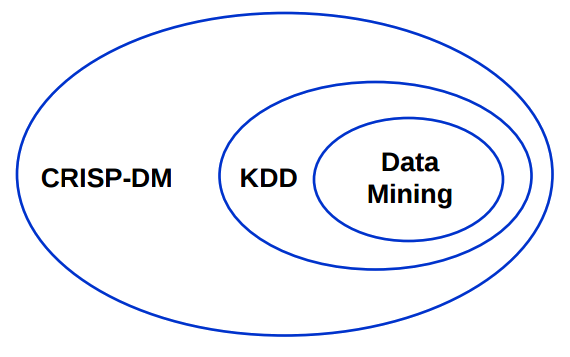
\includegraphics[width=90mm, height=40mm]{Figuras/RelacaoCrispKddDm.png}\\
\tiny Fonte: Neurotech -- 2012
\end{figure}

O modelo de processo CRISP–DM provê seis fases para um projeto de
mineração de dados, sendo assim determina-se um ciclo de vida
compreendido para cada uma dessas fases:
A primeira fase, conhecida como Entendimento do negócio, ou “fase
de entendimento dos objetivos e dos requerimentos sob a perspectiva
do negócio” (CHAPMAN; KERBER; WIRTH et al, 2000, p.10) é
uma fase crucial da mineração.
A segunda fase, Entendimento dos dados, caracteriza-se pelo exame
acurado dos dados, procurando identificar a sua qualidade. Dados
ausentes – “missing data” – são comuns em bases de dados não
estruturadas, configurando-se como um problema a ser considerado,
pois seu tratamento pode consumir muito tempo do analista de dados.
A terceira fase, Preparação dos dados, diz respeito à construção final
do conjunto de dados. Preparar os dados significa criar e selecionar
atributos, criar tabelas ou planilhas e registros dos dados.
Na quarta fase, Modelagem de I.A., a tecnologia deve ser escolhida de
forma criteriosa, baseada na experiência do analista de dados. Em
sistemas de suporte à decisão, uma tecnologia inadequada pode levar a
decisões imprecisas. É comum retornar às fases anteriores para
adequar a técnica aos dados.
Na fase cinco, Avaliação de desempenho, um ou muitos modelos
devem ter sido construídos e testados, de forma que seja possível
atingir uma alta qualidade do ponto de vista da análise dos dados, ou
seja, que o modelo proposto esteja adequado aos objetivos do
negócio.
A sexta e última fase, caracteriza-se pela conclusão do modelo. No
entanto, a criação do modelo não é o fim do processo. O conhecimento
adquirido precisa ser incrementado, podendo, inclusive, ser retomado
o ciclo até que o modelo esteja adequado às necessidades e
especifidades definidas previamente.

A figura a seguir ilustra as fases do ciclo:

\begin{figure}[!ht]
\centering
\caption{O padrão CRISP-DM \cite{Crisp2000}}
\vspace{1mm}
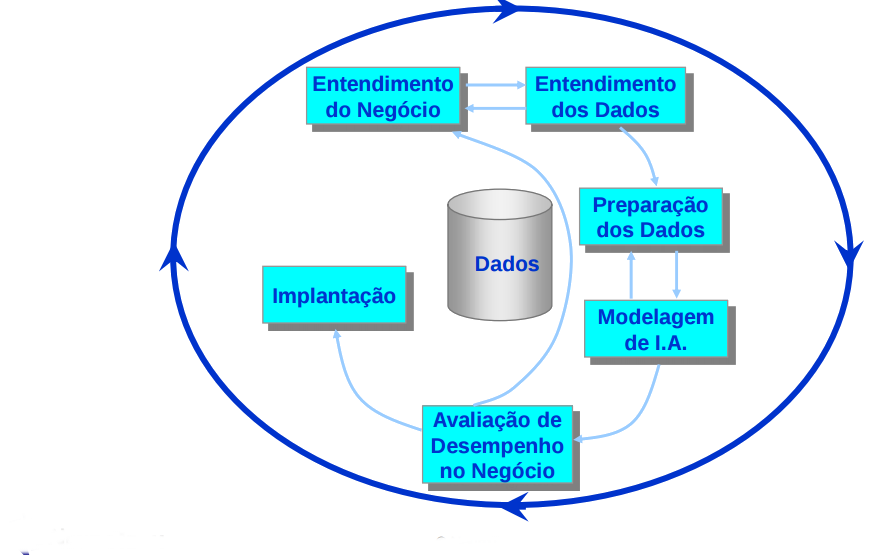
\includegraphics[width=70mm, height=60mm]{Figuras/CrispDM.png}\\
\tiny Fonte: CRISP-DM 1.0
\end{figure}


\subsection{Aprendizagem de Máquina - ``Machine Learning''}

Aprendizagem de Máquina ou ``Machine Learning'' são métodos para analisar dados de forma automatizada e interativa.
Segundo Shalev-Shwartz \& Ben-David \cite{Ben-David2014}, o termo Aprendizagem de Máquina refere-se à detecção automatizada de Padrões de dados.

Para Nilsson \cite{Nilsson2005}, o aprendizado ocorre quando uma máquina modifica sua estrutura interna, programa ou dados 
(baseados nos inputs ou em uma resposta para informação externa) de tal maneira que melhora o desempenho futuro.

Sistemas que executam tarefas de inteligência artificial, tais como Reconhecimento de Padrões, Diagnóstico, Controle de Robôs, Predição e 
outros, precisam ser modificados para executarem ``Machine Learning'' \cite{Nilsson2005}.

Historicamente, os tipos de aprendizagem computacional estão relacionados em ``o que'' há para ser aprendido \cite{Nilsson2005}. 
Primeiramente, para escolher o que aprender, é necessário definir de ``onde'' ou sobre quais dados aprender.
Deve-se fornecer um conjunto de treinamento para depois testar o conhecimento aprendido em um conjunto de teste.

Técnicas de mineração agrupam de dados de acordo com sua funcionalidade \cite{DataMining2}, que tem como característica principal a maneira como 
são descobertos os padrões no dados, podendo estar em uma das duas categorias: tarefas descritivas ou tarefas preditivas. 
As tarefas de mineração descritivas preocupam-se as características dos dados no conjunto de dados: o ``data set''. 
As preditivas, por sua vez, induzem regras nos dados correntes para produzirem de modo a produzir predições \cite{DataMining2}. 
O tópico a seguir analisa as tarefas preditivas.

\subsubsection{Classificação e Regressão para análise preditiva}

Classificação é um processo para encontrar um modelo que descreve e distingue classes de dados. 
Esse modelo tem como base de análise um conjunto de treinamento (i.e. objetos de dados para os quais 
serão encontrados rótulos que os classifiquem). 
Esse modelo é usado para predizer quais rótulos de classes terão os objetos desconhecidos.
O modelo pode ser representado por regras de classificação do tipo ``IF - THEN'', por árvores de decisão, redes neurais e outros. 
Regras de classificação se distinguem de regras de indução da seguinte forma:
\begin{itemize}
 \item Uma regra de classificação poderia ser: $if$ L $them$ class = $C_{1}$ ou $if$ L $them$  $C_{1}$
 \item Uma regra de indução seria: $ if$ L $them$ R que por sua vez produz novas regras 
\end{itemize}

As árvores de decisão são estruturas como fluxogramas, possuem nós e ramificações, 
cada nó é um teste no valor do atributo como:
\singlespace

\begin{figure}[ht] \unitlength= 1mm \thicklines
 \centering{
    \begin{picture}(90,6)%115
      \put(0,0){\framebox(86,6)} \put(3,2){\small $age(X,youth)$ AND $income(X,``high'')  \to classe (X,``A'')$}
      \put(0,-7){\framebox(85,6)} \put(3,-5){\small $age(X,youth)$ AND $income(X,``low'') \to classe (X,``B'')$}
      \put(0,-14){\framebox(71,6)} \put(3,-12){\small $age(X,``middle-aged'')$  $\to classe (X,``B'')$}
      \put(0,-21){\framebox(55,6)} \put(3,-19){\small $age(X,``senior'')$  $ \to classe (X,``B'')$}
      \end{picture}
   }
\end{figure}


\vspace{5mm}
  
A seguir, a árvore de decisão que explicita se um cliente, de acordo com sua idade terá determinada classe:
\begin{figure}[!ht]
\centering
\caption{Árvore de decisão}
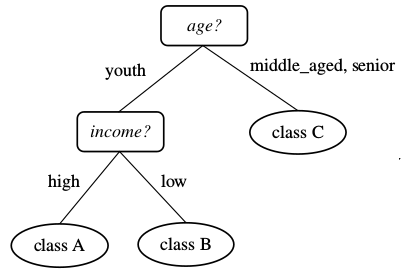
\includegraphics[width=50mm, height=35mm]{Figuras/arvorejovem.png}\\
\tiny Fonte: Han, J. and Kamber, M. 
\end{figure}  


A figura a seguir representa uma rede neural com as mesmas características da árvore de decisão anterior:
\begin{figure}[!ht]
\centering
\caption{Rede Neural}
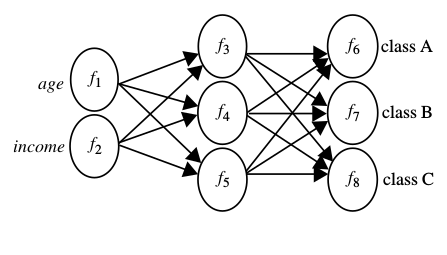
\includegraphics[width=65mm, height=28mm]{Figuras/redeneural.png}\\
\tiny Fonte: Han, J. and Kamber, M. 
\end{figure}  

As árvores de decisão são algoritmos rápidos que produzem regras de indução, contudo dados impuros podem comprometer o desempenho desse algoritmo. 
A fase de extração dos dados é fortemente influenciada pelas variáveis escolhidas, \cite{DecisionTree} 
isso pode representar o desafio maior para implementar esta técnica.

Outro problema que pode ser encontrado em algoritmos de aprendizagem é o ``overfitting'' ou superadaptação aos modelos.
Segundo RUSSEL E NORVIG (2004) o ``overfitting'' ocorre quando o número atributos é grande.

\subsubsection{Árvores de decisão - ``Decision Tree''}

Uma \textbf{árvore de decisão} tem como entrada um conjunto de \textbf{atributos} ou de variáveis para retornar como saída uma \textbf{decisão}.
O valor esperado da saída deve estar de acordo com o que foi dado à entrada.


Han e Kamber \cite{DataMining} definem indução por árvore de decisão como a aprendizagem de árvore de decisão a partir de classes rotuladas nas tuplas de treinamento. 
A estrutura da árvore de decisão é semelhante a um fluxograma, onde cada nó interno (não-folha) indica um teste de atributo, cada ramo representa o resultado de um teste e 
cada nó da folha possui um rótulo de classe. O nó de nível mais superior é chamado de nó-raiz.


Para Ian e Frank \cite{MachineLearning}, as árvores de decisão podem ser representadas por uma abordagem ``dividir para conquistar'' para resolução de problemas de 
aprendizagem, a partir de um conjunto de instâncias independentes. Os nós em uma árvore de decisão ``testam'' um atributo específico, comparando seu valor com uma constante.
No entanto, algumas árvores podem comparar dois atributos com outros ou utilizarem uma função para tal.
As árvores de decisão podem ser classificadas em dois tipos: árvores de regressão (regression trees), que são utilizadas para estimar atributos numéricos, e árvores de 
classificação (classification trees), usadas para análise de variáveis categóricas.
 

O algorítimo \textit{C4.5} é considerado um exemplo clássico de método de indução de árvores de decisão. O \textit{C4.5} \cite{Learning2007} foi inspirado no algoritmo 
\textit{ID3} \cite{Learning1979}, que produz árvores de decisão a partir de uma abordagem recursiva de particionamento de um conjunto de dados, utilizando conceitos e medidas 
da Teoria da Informação \cite{TeoriaInf}.

As árvores de decisão têm uma característica peculiar: a saída do modelo de predição (o output), com regras se -- então, é claramente perceptível por analistas humanos.
Essa qualidade é utilizada para interpretar os resultados.


\section{Desenho metodológico proposto}

O desenho metodológico proposto para o estudo contemplou as fases do KKD, conforme descrito a seguir.

\textbf{Target Data}: Nessa etapa foram coletadas as informações provenientes da base de dados da Polícia Rodoviária Federal (PRF) de 2007 a 2015, 
uma vez que nosso interesse era o de analisar os últimos dez anos. No entanto, como a base de dados só dispunha de informações a partir 
de 2007, foram considerados os nove anos disponíveis. A PRF dispunha de duas bases de dados distintas: a primeira contendo relatório de 
``acidentes'' e a outra, interdições. A partir dos dados capturados na base da PRF, utilizamos como variáveis de entrada: 
(1) nomenclatura da rodovia (i.e. BR 101); 
(2) quilômetro (km) em que se deu a ocorrência; 
(3) tipo de veículo envolvido na ocorrência: carro, motocicleta, caminhão, bicicleta, etc.; 
(4) tipo de acidente: colisão-frontal, lateral, traseira; atropelamento: com ou sem morte, envolvendo pessoas e/ou animais; 
(5) causa do acidente: ausência ou baixa visibilidade, excesso de velocidade, buracos na via, dentre outros; 
(6) horário e data da ocorrência; dentre outros que serão apresentados mais adiante. 

\textbf{Preprocessing}: nessa fase foram tomadas as variáveis, sendo desconsiderados alguns atributos, pelo fato de conterem inconsistências e 
missing data, como, por exemplo, informações acerca de latitude e longitude. Cabe destacar que a base, como um todo, apresentava sérias 
inconsistências, uma vez que, por exemplo, um mesmo acidente, quando envolvia dois ou mais veículos, era lançado na base duas ou mais 
vezes, em função da quantidade de veículos envolvidos. Foram eliminadas variáveis em duplicidade (i.e. as variáveis mês e ano, que apareciam 
separadamente, já estavam contempladas na variável Data.).
\textbf{Transformation}: Foram criadas as variáveis ``tipo de paralisação'', contemplando acidentes sem mortos e com, no máximo, 
dois veículos envolvidos; ``Dias da semana'' (sunday, mondai, …., saturado); ``Ajuste de hora'' (i.e. 17h58, 17h59, 18h, 18h01, 18h02, 
arredondadas para 18h); ``Ajuste de Km'' (seguindo a mesma lógica do ajuste de hora).
\textbf{Data Mining}: O algoritmo escolhido para o estudo foi a árvore de decisão, que possibilita uma interpretação imediata e de fácil 
compreensão. Como ferramentas, foram escolhidas o Knime e o Weka, com o objetivo de estabelecer uma comparação entre ambos, cuja intenção 
era a de produzir um classificador mais preciso. Nessa direção, a técnica Ensemble afirma que o produto de um ou mais classificadores 
iguais, ou mais de um classificador, aumenta a precisão. Tanto na ferramenta Knime quanto Weka a árvore de decisão é chamada J48, uma vez 
que se trata de uma implementação em java do algoritmo C4.5. Foi calculada a correção entre linear entre as variáveis ``tipo de acidente'' 
e ``traçado da via''.
\textbf{Interpretation/Evaluation}: Produção de árvores de decisão a partir do estabelecimento de diferentes nós-raízes, definidos em 
virtude da correlação linear encontrada.

\section{Dados de encontrados antes da Mineração}

%% BR 101 
\begin{figure}[ht]
\begin{center}
     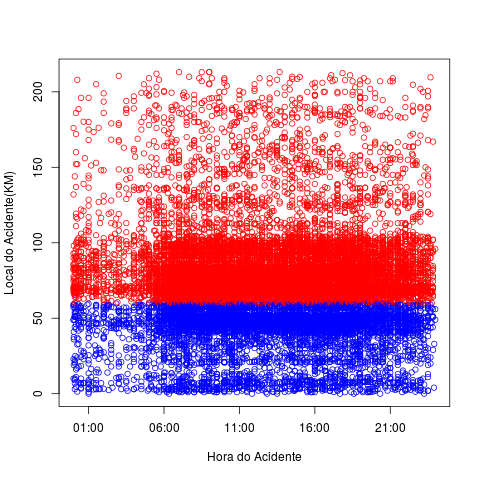
\includegraphics[height=4.0cm]{graficos/br101_1.png}
     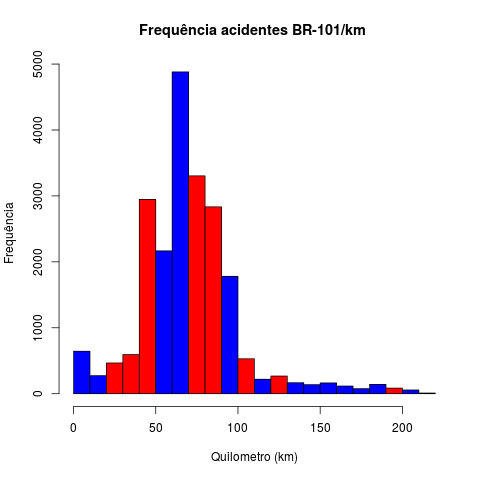
\includegraphics[height=4.0cm]{graficos/br101_2.png}
     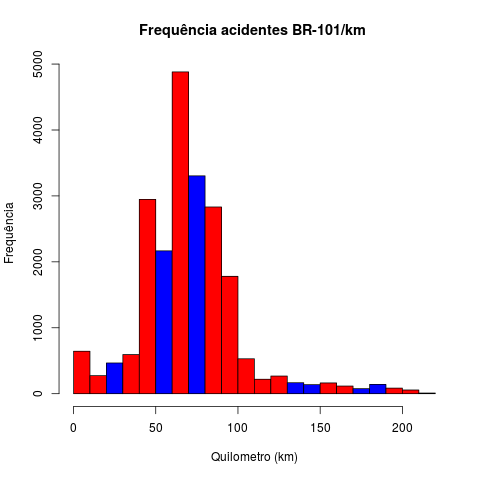
\includegraphics[height=4.0cm]{graficos/br101_3.png}
     \small{\caption{Graphic: hour x crash(km)-Road:BR 101}}
     \small{\caption{Boxplot: Período do dia}}
     \small{\caption{Histogram: place(Km) x frequence}}
\end{center}
\end{figure}

%% BR 104
\begin{figure}[ht]
\begin{center}
     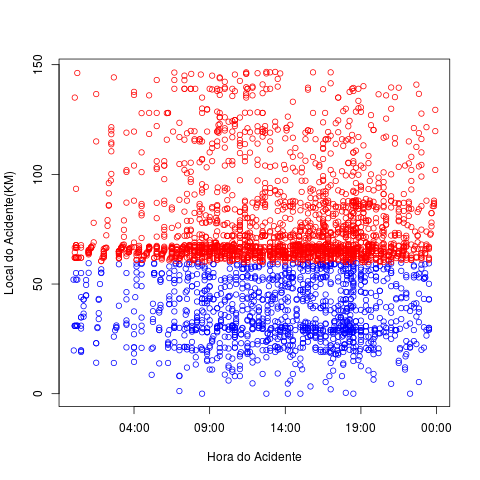
\includegraphics[height=4.0cm]{graficos/br104_1.png}
     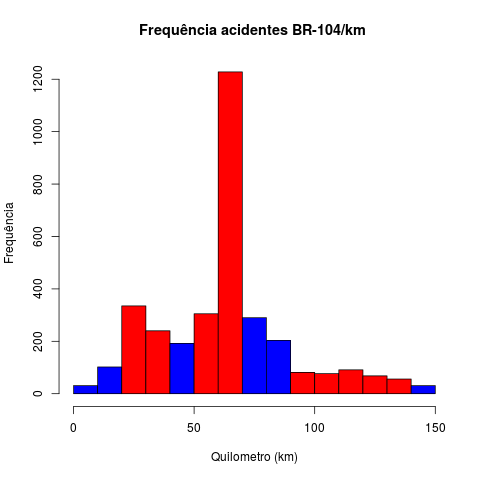
\includegraphics[height=4.0cm]{graficos/br104_3.png}
	\caption{Graphic: hour x crash(km)-Road:BR 104}
	\caption{Histogram: place(Km) x frequence}
\end{center}
\end{figure}

%% BR 110
\begin{figure}[ht]
\begin{center}
     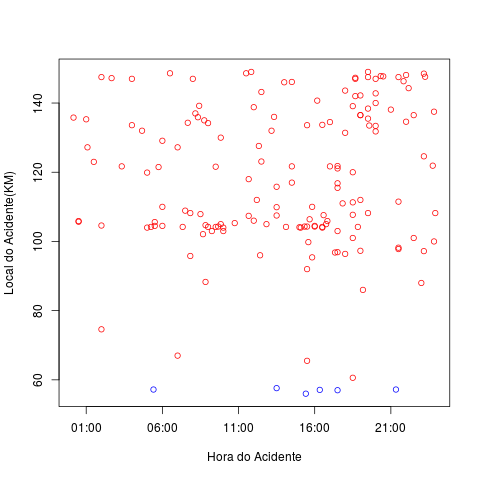
\includegraphics[height=4.0cm]{graficos/br110_1.png}
     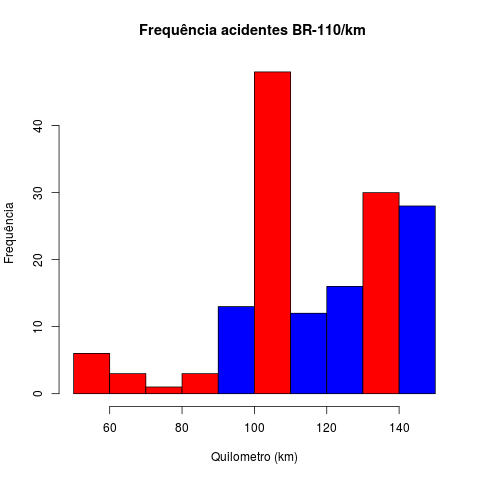
\includegraphics[height=4.0cm]{graficos/br110_3.png}
      \caption{Graphic: hour x crash(km)-Road:BR 110}
      \caption{Histogram: place(Km) x frequence}
\end{center}
\end{figure}

%% BR 116
\begin{figure}[ht]
\begin{center}
     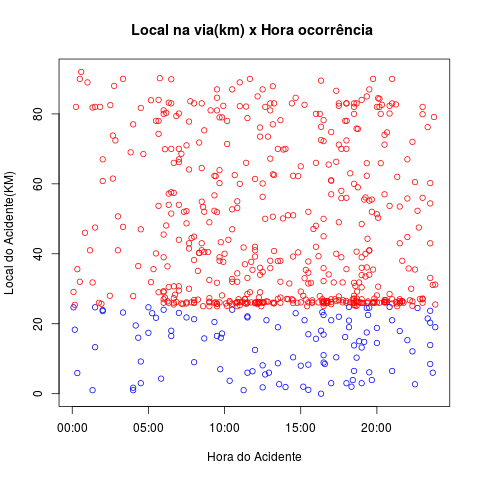
\includegraphics[height=4.0cm]{graficos/br116_1.png}
     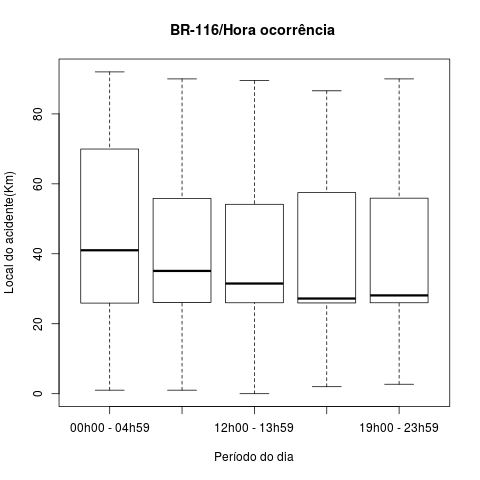
\includegraphics[height=4.0cm]{graficos/br116_2.png}
      \caption{Graphic: hour x crash(km)-Road:BR 116}
      \caption{Histogram: place(Km) x frequence}
\end{center}
\end{figure}

%% BR 232
\begin{figure}[ht]
\begin{center}
     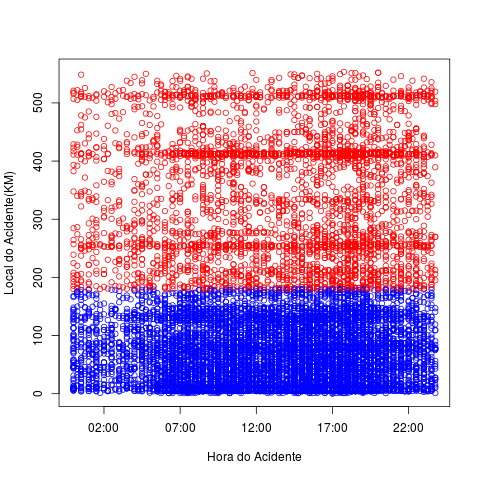
\includegraphics[height=4.0cm]{graficos/br232_1.png}
     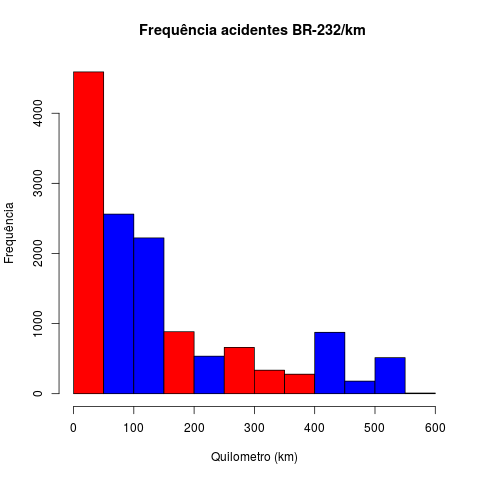
\includegraphics[height=4.0cm]{graficos/br232_2.png}
      \caption{Graphic: hour x crash(km)-Road:BR 232}
      \caption{Histogram: place(Km) x frequence}
\end{center}
\end{figure}

%% BR 316
\begin{figure}[ht]
\begin{center}
     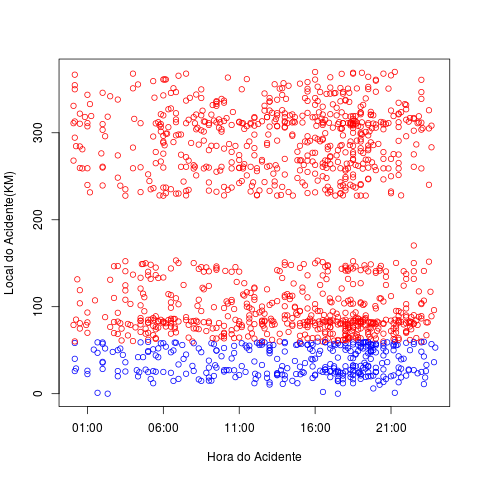
\includegraphics[height=4.0cm]{graficos/br316_1.png}
     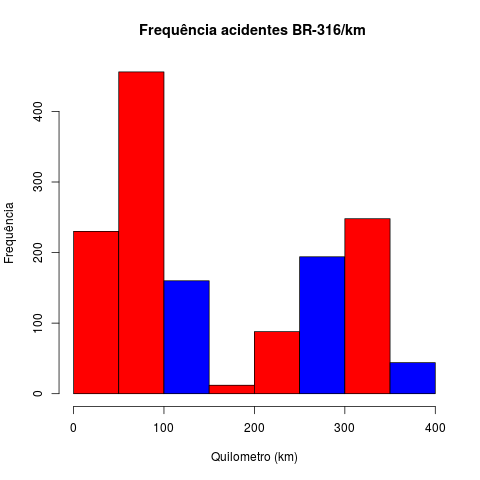
\includegraphics[height=4.0cm]{graficos/br316_2.png}
      \caption{Graphic: hour x crash(km)-Road:BR 316}
      \caption{Histogram: place(Km) x frequence}
\end{center}
\end{figure}

%% BR 407
\begin{figure}[ht]
\begin{center}
     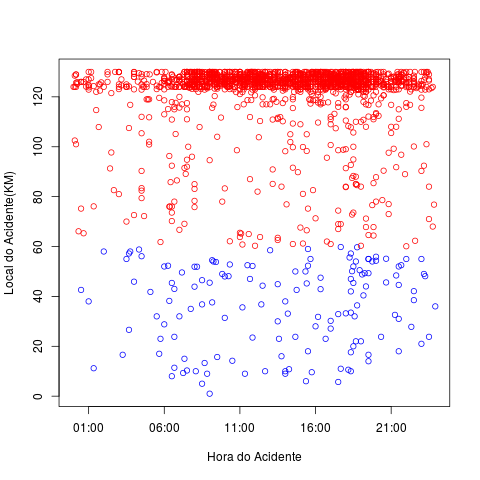
\includegraphics[height=4.0cm]{graficos/br407_1.png}
     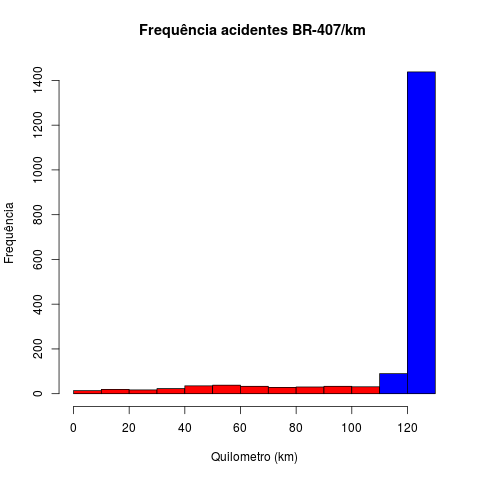
\includegraphics[height=4.0cm]{graficos/br407_2.png}
      \caption{Graphic: hour x crash(km)-Road:BR 407}
      \caption{Histogram: place(Km) x frequence}
\end{center}
\end{figure}

%% BR 408
\begin{figure}[ht]
\begin{center}
     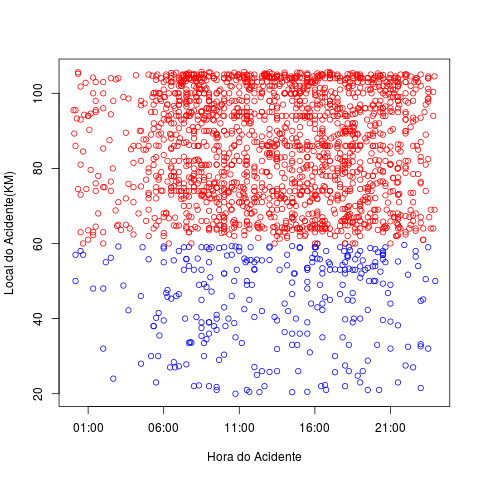
\includegraphics[height=4.0cm]{graficos/br408_1.png}
     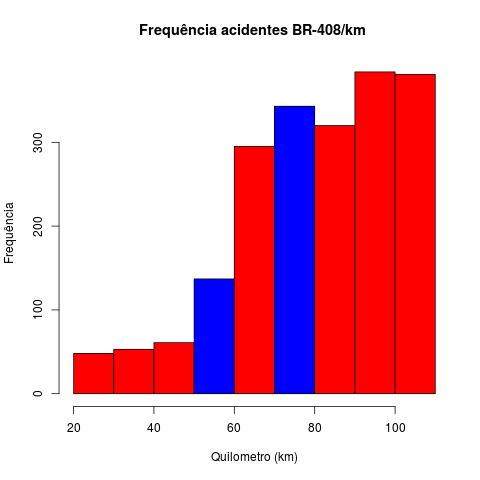
\includegraphics[height=4.0cm]{graficos/br408_2.png}
      \caption{Graphic: hour x crash(km)-Road:BR 408}
      \caption{Histogram: place(Km) x frequence}
\end{center}
\end{figure}

%% BR 423
\begin{figure}[ht]
\begin{center}
     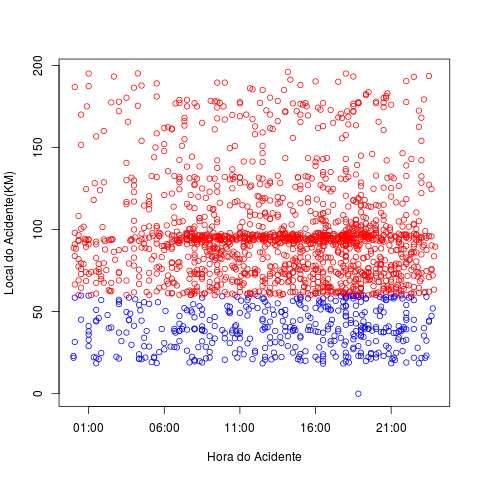
\includegraphics[height=4.0cm]{graficos/br423_1.png}
     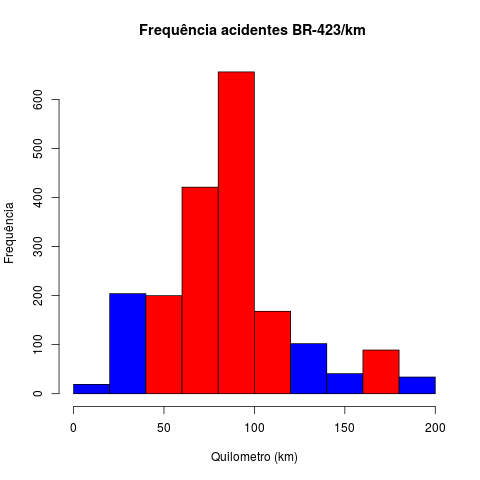
\includegraphics[height=4.0cm]{graficos/br423_2.png}
     \tiny{\caption{Graphic: hour x crash(km)-Road:BR 423}}
     \tiny{ \caption{Histogram: place(Km) x frequence}}
\end{center}
\end{figure}

%% BR 424
\begin{figure}[ht]
\begin{center}
     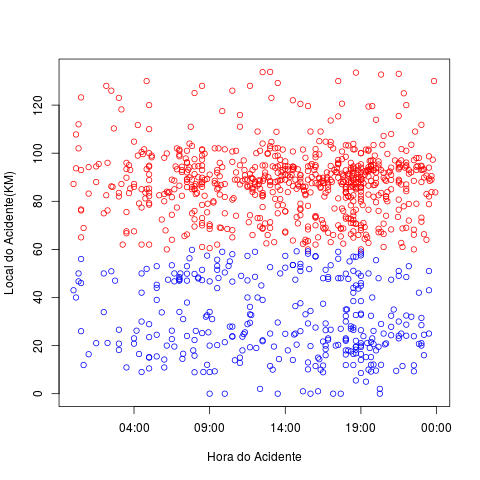
\includegraphics[height=4.0cm]{graficos/br424_1.png}
     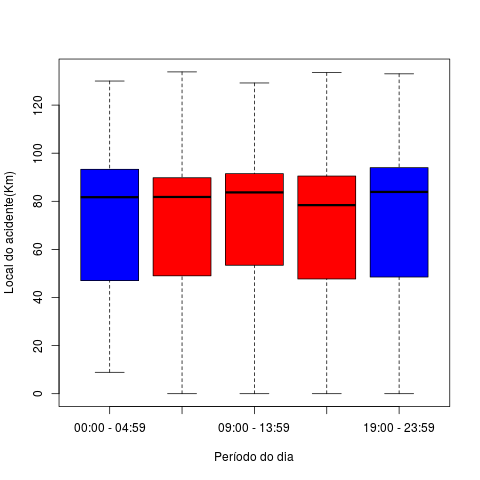
\includegraphics[height=4.0cm]{graficos/br424_2.png}
     \small{\caption{Graphic: hour x crash(km)-Road:BR 424}}
     \small{\caption{Histogram: place(Km) x frequence}}
\end{center}
\end{figure}

%% BR 428
\begin{figure}[ht]
\begin{center}
     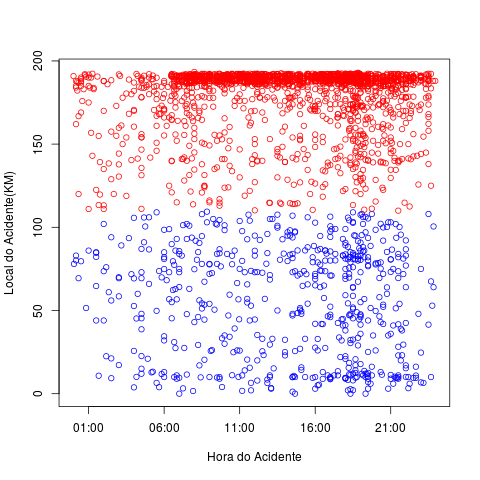
\includegraphics[height=4.0cm]{graficos/br428_1.png}
     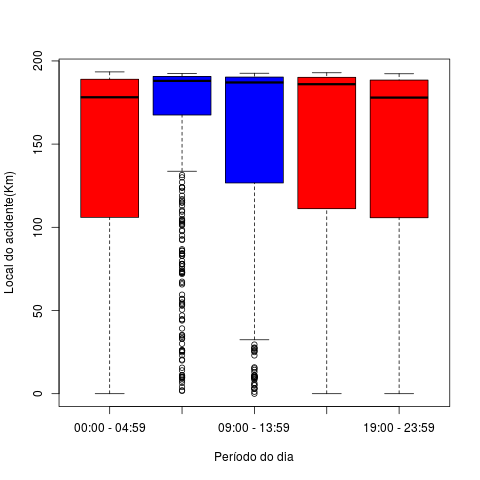
\includegraphics[height=4.0cm]{graficos/br428_2.png}
     \tiny { \caption{Graphic: hour x crash(km)-Road:BR 428}}
     \tiny { \caption{Histogram: place(Km) x frequence}}
\end{center}
\end{figure}


\section{Dados depois da Mineração}

\pagebreak


\section{Considerações finais}

A contribuição dessa pesquisa é de cunho metodológico-prático.
Do ponto de vista metodológico pela aplicação do processo CRISP-DM, usado para construir o modelo preditivo; do ponto de vista prático 
pela proposição de um modelo que integre predição à API de mapas de posicionamento global, fornecendo informação suficiente a um gestor para decidir quando 
e por onde enviar uma frota de caminhões por determinada rodovia que apresente retenções crescentes de logística de cargas. 

As soluções disponíveis que existem tais como; Google Maps, Waze e outros dessa natureza somente exibem informações momentâneas, produzidas e compartilhadas pelos utilizadores 
dos aplicativos ou por informações provindas de GPS, contudo não analisam dados históricos dessas rodovias nem fazem predições sobre o seu comportamento.

Outra contribuição dessa pesquisa é a proposição de um arco cibernético construído com a API de redes sociais.
Os ``feeds'' de notícias das redes sociais como o Twitter permitem analisar o contexto das rodovias com defasagem temporal muito pequena.
Os utilizadores dessas redes sociais contribuem com muita informação relevante como por exemplo o anúncio de uma paralisação que ocorrerá 
daqui a uma semana, a PRF de Pernambuco é outro contribuidor permanente; com seu canal no Twitter: @PRF191PE fornece diariamente informação das rodovias 
além de dados estatísticos. 

A monitoração de redes sociais é feita por Mineração de dados em textos, em que são verificas palavras chaves tais como: protestos, acidentes, paralisação, no caso
específico do nosso estudo.

Uma vez capturadas e tratadas, as informações desses ``feeds'' são direcionadas a um banco de dados. 
Foi escolhido o Sistema Gerenciador de Banco de Dados (SGBD) MySQL para tratar esses ``feeds'' do Twitter. 
A opção pelo MySQL foi devido às características que consideramos essenciais, tais como: licença para livre utilização, boa capacidade para gerenciar grande quantidade de 
dados e por seguir o padrão SQL-ANSI; portanto não foi necessário estudo mais aprofundado para operacionalizar; ``select'', ``insert'' e ``update''.


% conference papers do not normally have an appendix



% use section* for acknowledgment
\ifCLASSOPTIONcompsoc
  % The Computer Society usually uses the plural form
  \section*{Acknowledgments}
\else
  % regular IEEE prefers the singular form
  \section*{Acknowledgment}
\fi


The authors would like to thank...




\begin{thebibliography}{1}

%1
\bibitem{Bitoun2012}
  J. Bitoun, and L. Miranda, and M. A. Souza, et al
  title: {Regi\~{a}o Metropolitana do Recife no Contexto de Pernambuco no Censo 2010},
  pages: {25},
  url:   {http://www.observatoriodasmetropoles.net/download/Texto\_BOLETIM\_RECIFE\_FINAL.pdf},
  Acessado em: {17 abril. 2016},
  year:  {2012}

  
\bibitem{FrotaVeiculosIBGE}
  Instituto Brasileiro de Geografia e Estatística - IBGE,
  title: {Região Metropolitana do Recife no Contexto de Pernambuco no Censo 2010},
  url:  {http://www.cidades.ibge.gov.br/painel/frota.php},
  Acessado em: {17 abril. 2016},
  year = {2014}



\bibitem{Fayyad}
  P., Fayyad, U., Piatetsky-Shapiro, G \& Smyth,
  booktitle: {From data mining to knowledge discovery in databases. Advances in Knowledge Discovery and Data Mining}
  doi: {10.1609},
  volume: {17(3)},
  pages: {1–36},
  year: {1996}

%2
\bibitem{Castanheira}
  L., G., Castanheira,
  title: {Aplicação de Técnicas de Mineração de Dados em Problemas de Classificação de Padrões},
  number: {5531},
  year: {2013}
  
  
%3
\bibitem{bigdataQualquerUm}
  H. V. Jagadish, J. Gehrke, A. Labrinidis, Y. Papakontantinou, J. M. Patel, R. Ramakrishnan and C. Shahabi,
  booktitle: {Exploring the inherent technical challenges in realizing the potential of Big Data},
  publisher: {journal:Comunication of the ACM}, 
  volume: {57,r7}, 
  pages: {86--96}, 
  month: {July}, 
  year: {2014}

  
\bibitem{Learning2007}
  J. R. Quinlan,
  title = {Induction of Decision Trees},
  doi = {10.1023/A:1022643204877},
  isbn = {0885-6125},
  issn = {0885-6125, 1573-0565},
  journal = {Expert Systems},
  publisher = {Learning, Machine and Learning, Machine and Publishers},
  pages = {81--106},
  pmid = {17050186},
  year = {2007}


%[32]
\bibitem{Learning1979}
  J. R. Quinlan,
  title = {Discovering rules by induction from large collections of examples},
  journal = {Expert systems in the micro electronic age. Edinburgh University Press},
  publisher = {In D. Michie},
  year = {1979}

  
\bibitem{TeoriaInf}	
  Han, J and Kamber, M,
  title = {Data mining: concepts and techniques},
  volume = {2nd editio},
  year = {2006}

  
\bibitem{DataMining}
  J. Han, and M. Kamber,
  title = {Data Mining: Concepts and Techniques},
  publisher = {Elsevier, San Francisco},
  volume = {2 edition},
  year = {2006}


\bibitem{MachineLearning}
  Ian H. Witten and Eibe Frank,
  title = {Data Mining: Practical Machine Learning Tools and Techniques},
  journal={Elsevier, San Francisco},
  volume ={2 edition},
  year = {2005}

  
%4
\bibitem{DataMining2}
  J. Han, and M. Kamber,
  title: {Data Mining: Concepts and Techniques},
  publisher: {Elsevier, San Francisco},
  pages: {15--16},
  volume: {2 edition},
  year: {2006}

  
\bibitem{Chapman2000}
  P. Chapman, and J. Clinton, and R. Kerber, and T. Khabaza et al,
  title: {Crisp-Dm 1.0},
  publisher: {CRISP-DM Consortium},
  pages: {76},
  year: {2000}

\bibitem{Crisp2000}
  R. Wirth,
  title: {CRISP-DM 1.0 – Step-by-step data mining guide},
  pages: {7--10},
  year: {2000}

  
\bibitem{possas1998data}
  B. POSSAS, and M.L.B. CARVALHO, and R.S.F. REZENDE, and W. MEIRA JR,
  title: {Data mining: t{\'e}cnicas para explora{\c{c}}{\~a}o de dados},
  journal: {Universidade Federal de Minas Gerais},
  year: {1998}

  
  
\bibitem{Ben-David2014}
  S. Ben-David, and S. Shalev-Shwartz,
  title: {Understanding Machine Learning: From Theory to Algorithms},
  booktitle: {Understanding Machine Learning: From Theory to Algorithms},
  doi: {10.1017/CBO9781107298019},
  isbn: {9781107057135},
  pages: {449},
  url: {http://www.cs.huji.ac.il/{~}shais/UnderstandingMachineLearning/understanding-machine-learning-theory-algorithms.pdf},
  year: {2014}

  

\bibitem{Nilsson2005}
  J. N. Nilsson,
  title: {Introduction to Machine Learning},
  doi: {10.1016/j.neuroimage.2010.11.004},
  eprint: {0904.3664v1},
  isbn: {9780262012430},
  issn: {10959572},
  journal: {Machine Learning},
  number: {2},
  pages: {387--99},
  pmid: {21172442},
  url: {http://www.ncbi.nlm.nih.gov/pubmed/21172442},
  volume: {56},
  year: {2005}  
  

%15
\bibitem{DecisionTree}
  A. Srivastava, V. Katiyar and N. Singh -- Review of Decision Tree Algorithm: Big Data Analytics,
  publisher: {Journal of Informative \& Futuristic Research},
  number = {10},
  pages = {3644--3654},
  volume = {2},
  year = {2015}
  
  
%6
\bibitem{singer}
SINGER, Talyta. TUDO CONECTADO: CONCEITOS E REPRESENTAÇÕES DA INTERNET DAS COISAS. 2012.
Acessado em: 23 abril. 2015.
\href{http://www.simsocial2012.ufba.br/modulos/submissao/Upload/44965.pdf} {Singer}

%7
\bibitem{Twitter2015}
Dorsey, J. Williams, B. Stone, E. and Glass, N.
Acessado em: 01 Julho de 2015
\href {https://pt.wikipedia.org/wiki/Twitter}
{Twitter}

%8
\bibitem{Filesystem}
  Filho, João Heriberto Mota,
  booktitle: {Descobrindo o Linux: entenda o sistema operacional GNU/Linux},
  isbn: {978-85-7522-278-2},
  pages: {153--162},
  year: {2012}




%10
\bibitem{Lange2015}
Lange, Benoit and Nguyen, Toan
title = {{A Hadoop use case for engineering data}},
mendeley-groups = {DataMiningBigData},
year = {2015}


%11
\bibitem{Dean2008}
Dean, Jeffrey and Ghemawat, Sanjay
institution = {Google, Inc.},
issn = {00010782},
journal = {Communications of the ACM},
number = {1},
pages = {1--13},
pmid = {11687618},
publisher = {ACM},
series = {SIGMOD '07},
title = {{MapReduce : Simplified Data Processing on Large Clusters}},
volume = {51},
year = {2008}
\href{http://portal.acm.org/citation.cfm?id=1327492}{MapReduce}


%12
\bibitem{Aranha2006}
Aranha, Christian and Passos, Emmanuel,
A Tecnologia de Mineração de Textos,
booktitle = {RESI-Revista Eletrônica de Sistemas de Informações},
doi = {10.5329/171},
issn = {1677-3071},
keywords = {Data minig,Intelligent information systems},
mendeley-groups = {Mineração Textos},
number = {2},
pages = {1--8},
volume = {2},
year = {2006}


%13
\bibitem{Amin2015}
Amin, Adnan and Faisal, Rahim and Imtiaz, Ali and Changez, Khan and Anwar, Sajid,
title = {{A Comparison of Two Oversampling Techniques (SMOTE vs MTDF) for Handling Class Imbalance Problem: A Case Study of Customer Churn Prediction}},
doi = {10.1007/978-3-319-16486-1},
isbn = {978-3-319-16485-4},
keywords = {big data,stock prediction,text mining},
mendeley-groups = {DataMiningBigData},
pages = {215--225},
volume = {353},
year = {2015},
\href{http://link.springer.com/10.1007/978-3-319-16486-1}{stockprediction}





%21
\bibitem{Baig2012}
Baig, Abdul Rauf and Shahzad, Waseem,
doi = {10.1007/s00521-010-0490-5},
title = {{A correlation-based ant miner for classification rule discovery}},
issn = {09410643},
journal = {Neural Computing and Applications},
keywords = {Ant colony optimization (ACO),Classification rules,Data mining,Swarm intelligence},
mendeley-groups = {DataMiningSwarnIntelligence},
number = {2},
pages = {219--235},
volume = {21},
year = {2012}


%14.1
\bibitem{motorBusca}
Fonte: Chaffey,
page = 378,
year=2006




%16
\bibitem{chambers2014computer}
W. D. Chambers (2014).
\emph{Computer simulation of dental professionals as a moral community. Medicine, Health Care and Philosophy}
\relax  17(3), 467–476.




%22
\bibitem{madeira}
Madeira, Lamont. Hoje a internet, amanhã os desafios da internet das coisas. 2011.

%23
\bibitem{mayumi}
MAYUMI, Danielle. Computação nas nuvens – O futuro da internet. 2011.



\end{thebibliography}






% that's all folks
\end{document}


